\documentclass{article}
%\url{https://tex.stackexchange.com/q/549289/86}
\usepackage{tikz}
\usetikzlibrary{braids}


\begin{document}

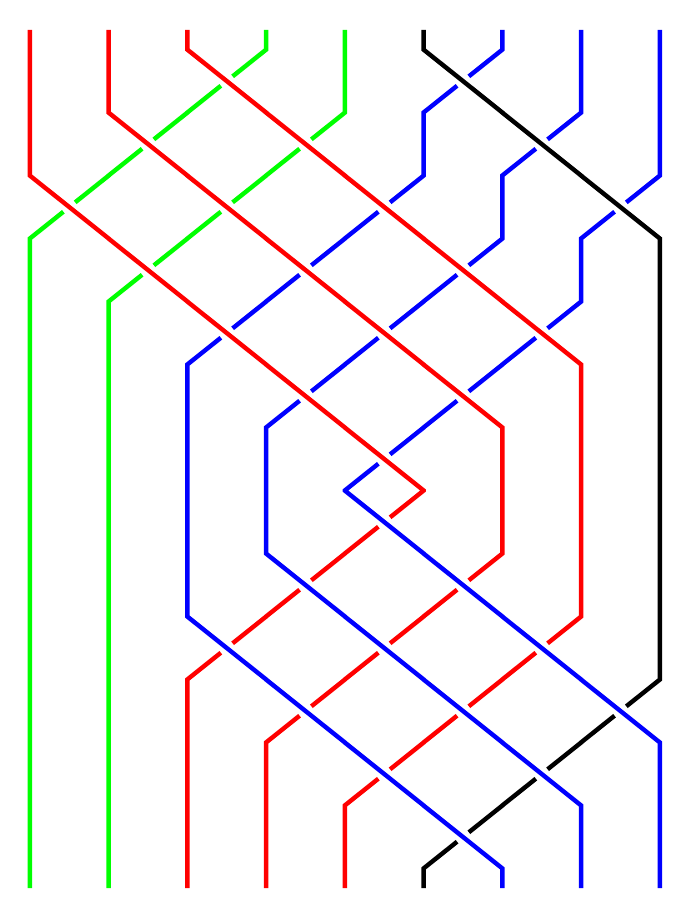
\begin{tikzpicture}
\pic[
  braid/.cd,
  every strand/.style={ultra thick},
  strand 1/.style={red},
  strand 2/.style={red},
  strand 3/.style={red},
  strand 4/.style={green},
  strand 5/.style={green},
  strand 6/.style={black},
  strand 7/.style={blue},
  strand 8/.style={blue},
  strand 9/.style={blue},
  control factor=.001,
  nudge factor=.001,
  height=-.8cm
  ]
{braid={%
s_3-s_6
s_2-s_4-s_7
s_1-s_3-s_5-s_8
s_2-s_4-s_6
s_3-s_5-s_7
s_4-s_6
s_5
s_5
s_4-s_6
s_3-s_5-s_7
s_4-s_6-s_8
s_5-s_7
s_6
}};
\end{tikzpicture}

\end{document}
